\documentclass[../main.tex]{subfiles}
\begin{document}

\begin{figure}
    \centering
    \begin{subfigure}[t]{0.2\textwidth}
        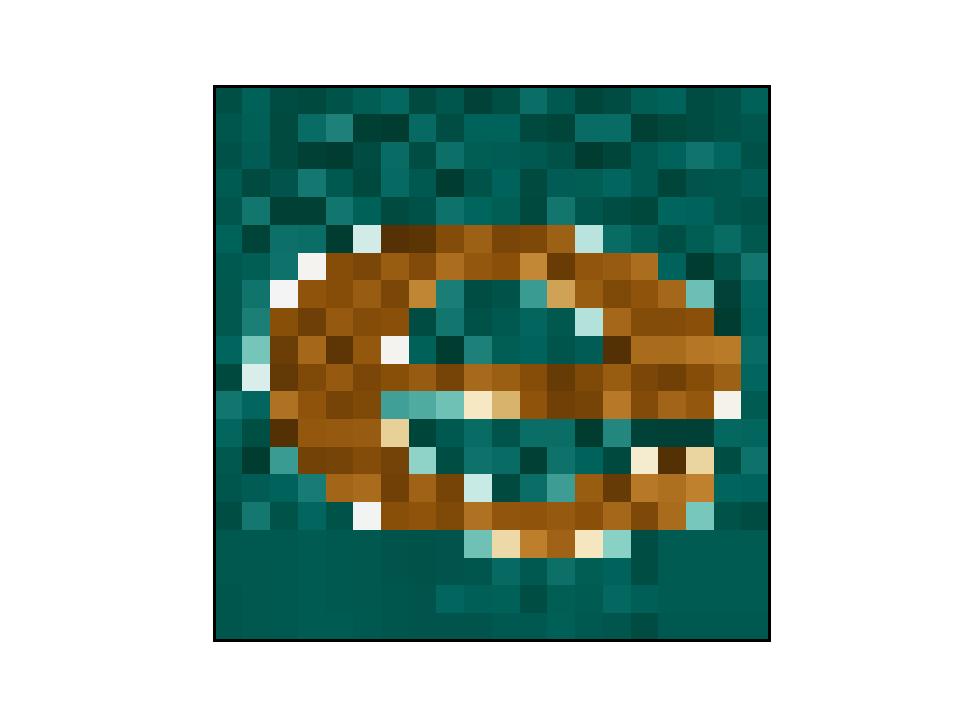
\includegraphics[width=\textwidth]{figures/pp/raw.pdf}
        \caption{Raw image.}
        \label{fig:gull}
    \end{subfigure}
    ~ %add desired spacing between images, e. g. ~, \quad, \qquad, \hfill etc. 
      %(or a blank line to force the subfigure onto a new line)
    \begin{subfigure}[t]{0.2\textwidth}
        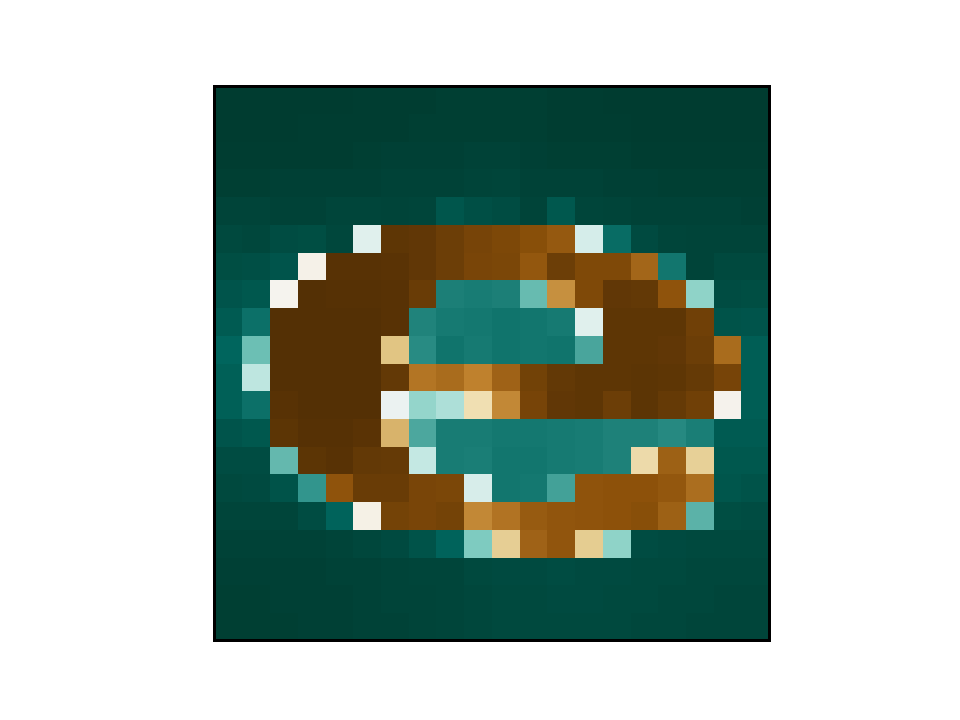
\includegraphics[width=\textwidth]{figures/pp/denoise.pdf}
        \caption{Denoised image.}
        \label{fig:denoise}
    \end{subfigure}
    ~ %add desired spacing between images, e. g. ~, \quad, \qquad, \hfill etc. 
    %(or a blank line to force the subfigure onto a new line)
    \begin{subfigure}[t]{0.2\textwidth}
        
\includegraphics[width=\textwidth]{figures/pp/img_to_bool.pdf}
        \caption{Binary image.}
        \label{fig:bool}
    \end{subfigure}
        ~ %add desired spacing between images, e. g. ~, \quad, \qquad, \hfill etc. 
    %(or a blank line to force the subfigure onto a new line)
    \begin{subfigure}[t]{0.2\textwidth}
        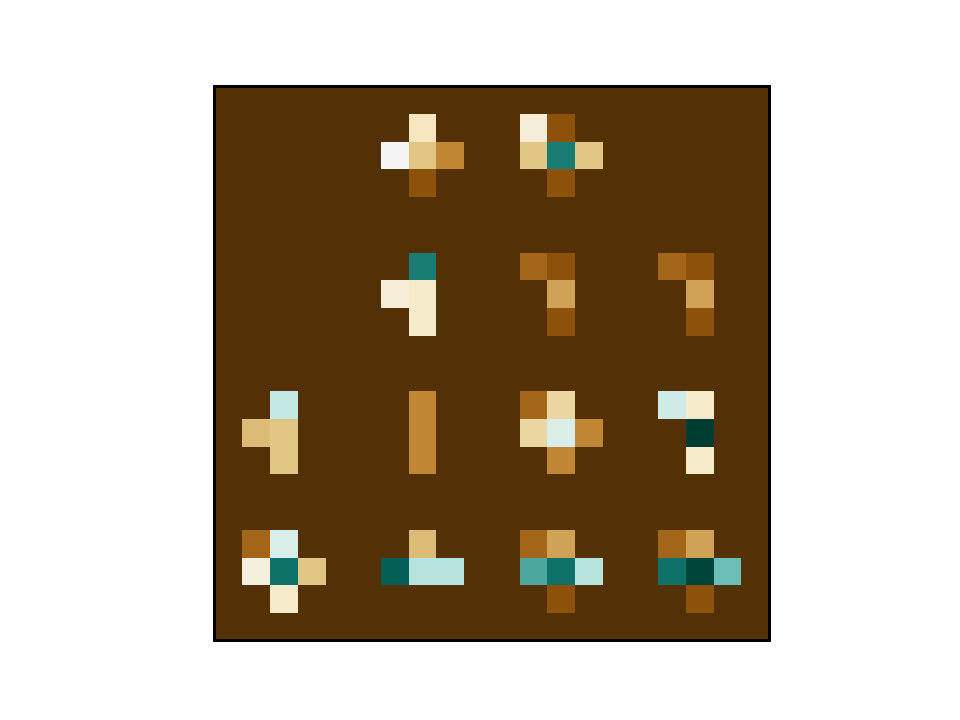
\includegraphics[width=\textwidth]{figures/pp/hog.pdf}
        \caption{Histogram of Oriented Gradients.}
        \label{fig:hog}
    \end{subfigure}
    \caption{Example of random selected image before and after preprocessing. The colors has been altered using a color map to visually enhance variance.}\label{fig:pp_image}
\end{figure}

In this section, the preprocessings of the images are shown and discussed. The preprocessing is preformed to enable easier classification for the classifier. Several preprocessing tools were explored to make the character easier to recognize for the classifier. The first preprocessing tool applied was total-variation denoising on n-dimensional images \cite{dnoise_tv_chambolle}. This technique reduces the total variation of an image. This is useful to avoid classifying noise, as the picture will now contain fewer components with high spacial frequency. An example of this denoising technique is shown in the image \autoref{fig:denoise}.

To increase contrast, we used Otsu's method, which is a way to perform image thresholding based on clustering \cite{otsu} automatically. After thresholding, the image was morphologically closed. This is a standard technique in image processing to remove small wholes in binary images. The result is shown in \autoref{fig:bool}. All though the result was visually pleasing; it did not decrease the error rate. Therefore, this method was discarded from further analysis.

The last preprocessing tool applied before dimention reduction was Histogram of Oriented Gradients. It is a feature descriptor uses local object appearences and shapes and describe them as a distribution of intensity gradients. It can be interpreted as the spacial derivative of the intencity of the image. The purpose of this step is to format the image for easier detection later as each element now carry more information than the pixels in the original.

One feature engineering method used and not covered by this section is Principal Component Analysis. Because its application is heavily based on the $k$-nearest neighbor algorithm, it will be covered in \autoref{sec:pca}.

\end{document}